\documentclass{sig-alternate}
\usepackage{color}
\usepackage[colorinlistoftodos]{todonotes}
\usepackage{graphicx}
\graphicspath{ {images/} }
\usepackage{mathtools}
\usepackage{amsmath}

\begin{document}
\conferenceinfo{UMM CSci Senior Seminar Conference, December 2015}{Morris, MN}

\title{Thermal Interaction In Spatial Augmented Reality}

\numberofauthors{1}

\author{
% The command \alignauthor (no curly braces needed) should
% precede each author name, affiliation/snail-mail address and
% e-mail address. Additionally, tag each line of
% affiliation/address with \affaddr, and tag the
% e-mail address with \email.
\alignauthor
Justin B. YaDeau\\
	\affaddr{Division of Science and Mathematics}\\
	\affaddr{University of Minnesota, Morris}\\
	\affaddr{Morris, Minnesota, USA 56267}\\
	\email{yadea003@morris.umn.edu}
}

\maketitle

\begin{abstract}
I will discuss two papers one paper goes over the use of thermal sensors to be able to utilize any real object with mobile technology and the other uses spatial augmented reality as a tool for 3D data visualization. Taking both of these ideas and putting them together is the goal of this paper. Imagine being able to interact with 3D data visualization, without having to actually touch an electronic device. This can reduce the amount of electronic devices needed for modern life.
\end{abstract}

\keywords{thermal interaction, 3D data visualization, augmented reality, AR, spatial augmented reality, SAR}

\section{Introduction}
\label{sec:Introduction}
Imagine being able to touch a table and have a phone know where was touched. Now think of the same scenario, but this time the phone says the number 0 was pressed because the area touched corresponded to the number 0 on a dial pad see figure \ref{fig:numpad}. Kurz \cite{Thermal} wrote a paper on this very topic. Being able to use thermal technology to accurately tell if a surface was touched by a finger and where. Kurz \cite{Thermal} states that as wearable technology becomes more prominent alternative solutions to touch screens will be sought after. With that in mind being able to interact with technology with a screen would help advance the wearable technology.    

Now think of a table that has a cone on it with projectors displaying data on cone. This is how Thomas et al. describes one of the ways to utilized spatial augmented reality as a tool for 3D data visualization (See figure \ref{fig:Tabletop}). Using technologies to track where the person being able to move the cone to define a new visualization. Also mentioning the scalability of the proposed system. CAVE systems would be the larger versions of the table top design mentioned above.      

I will discuss both and then joining them together in a way to minimizes the limitations that each has. Showing the possible applications that would be possible when joining these two methods.       


\section{Background}
\label{sec:background} 
Before starting this paper there are some concepts that should be made clear. It will be helpful to have a clear understanding of the differences between virtual reality, augmented reality and spatial augmented reality. Also knowing the concept of six degrees of freedom is beneficial.  

\subsection{Virtual Reality}
\label{sec:Virtual Reality}
Personally one of the more well known example of Virtual Reality (VR) today is the Oculus Rift. An earlier take on VR from Nintendo in the 90's is the Virtual Boy. Like the Oculus Rift the Virtual Boy is a device that strapped to the head of the user and used to simulate a virtual world mainly though sight. VR is nothing new another early example would be the view master, the stereoscopic toy that had circular inserts requiring the user to look into a light source to illuminate the picture. Being a more primitive the view masters still ''artificially creates sensory experiences, which can include sight, hearing, touch, and smell''\cite{VR}.       

\subsection{Augmented Reality}
\label{sec:Augmented Reality}
Augmented Reality (AR) can be described as augmenting the environment of the real world. It's different from VR because it is based in the physical world instead of the digital world. An example is Google Translate: using the camera from a phone, it translates foreign words that the camera is pointed at. Using a program it can detect words, mainly printed words, then using the roughly the same font and font size. Then the program overlays the translation onto the sign, billboard, or menu on the screen. Another example would be for anyone who bought a 3DS might the 3D cards the device came with the system, those are also a form of AR. A 3DS is a hand held gaming device that make the game being played 3D without the use of 3D glasses. The cards that came with the system were little mini games. Placing a card on the table, or any surface, and going into the application started a game. Creatures would pop up that you would fight, or trying to hit bulls-eye on target. All this is done on the surface the card was placed on.     

\subsection{Spatial Augmented Reality}
\label{sec:Spatial Augmented Reality}
Spatial Augmented Reality (SAR) is similar to AR. The difference is that it focuses more on augmenting reality through projection technology, instead of using conventional monitors or other such devices. A good example of SAR is if you have a sandbox with a topographical map overlaid onto the sand. You could move the sand around and the projector would be able to detect the height of the sand and match the peaks and valleys in the sand with the correct topographic overlay for displaying peaks and valleys. The way Thomas et al \cite{3D} defines SAR is 
\begin{quote}
Spatial Augmented Reality (SAR) enhances the visual aspects of physical objects, allowing users to better understand the virtual content. The users not only view the digital information but also gain a tactile understanding through touching the physical object.
\end{quote}

\subsection{6DOF}
\label{sec:6DOF}
6DOF, 6 degrees of freedom, are the different ways one can move in three dimensional space . From/back, left/right, up/down, roll, pitch, yaw are all the ways to move. Roll is moving clockwise or counter clockwise in relation to the front/back axis. Yaw is moving the front/back axis to either left/right axis. Pitch is the same yaw, except the up/down axis instead of the left/right axis. For any cerification see figure \ref{fig:6DOF}
\begin{figure}
	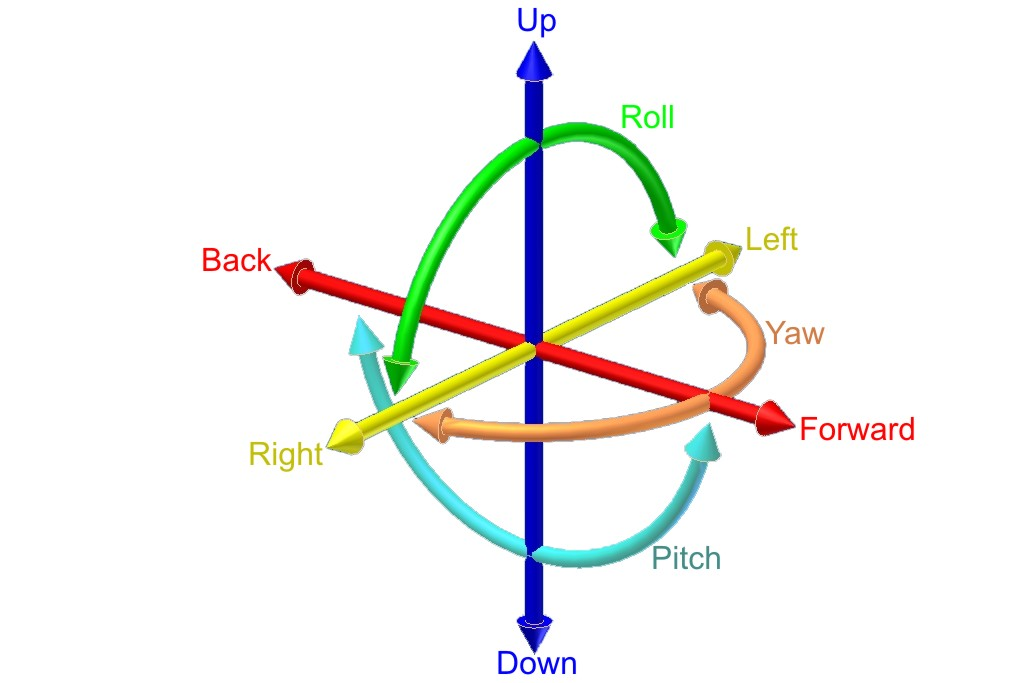
\includegraphics[width=8.5cm, height=5cm]{6DOF_en}
	\caption{Shows all the 6DOF axises \cite{6DOF}}
	\label{fig:6DOF}
\end{figure} 

\begin{figure}
	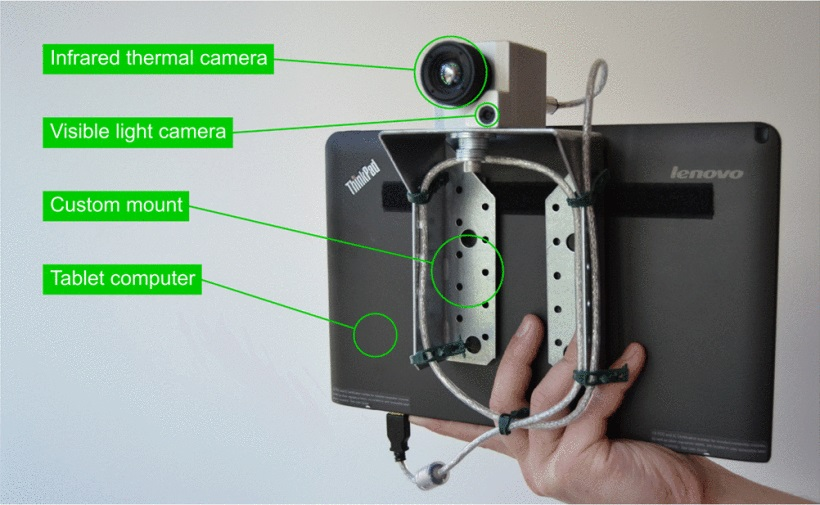
\includegraphics[width=8.5cm, height=5cm]{Hardware2}
	\caption{The hardware prototype used throughout Kurz's paper comprises a visible light camera and an infrared thermographic camera attached and connected to a tablet computer with a custom mount. \cite{Thermal}}
	\label{fig:hardware}
\end{figure} 
\begin{figure*}
	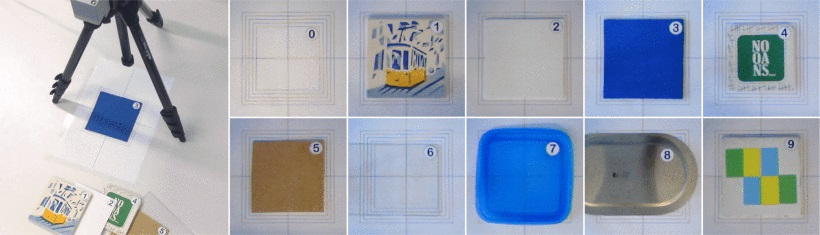
\includegraphics[width=18cm, height=5cm]{ThermalTesting}
	\caption{Different materials used in Kurz's evaluation: (0) paper on a plastic table top, (1) ceramic, (2) rigid PVC, (3) foam plastic, (4) cardboard, (5) laminated fiber sheet, (6) glass, (7) thin plastic, (8) steel, (9) multi-layer board. \cite{Thermal}}
	\label{fig:ThermalTest}
\end{figure*}
\section{Thermal Interaction}
\label{sec:Thermal Interaction}

Kurz \cite{Thermal} provides a way to interact with AR applications using objects or surfaces around everyday in everyday life. Using infrared thermography, his system can detect if the user touched a surface or came close to touching it. Keeping in mind one's finger(s) are warm and the surface is presumably cool, a touch leaves a heat signature on the cool surface. Kurz's system assumes that it takes place in a controlled environment where objects will be cooler then body temperature. When the thermal image detects a heat signature the same system is able to determine the 3D position on the touched physical object. 


\subsection{Hardware}
\label{Hardware}

The hardware that Kurz's \cite{Thermal} setup used a camera mounted to a tablet computer as shown in figure \ref{fig:hardware}. This needed to be custom fitted since the technology for thermal imagery is not readily built into everyday devices like tablets or phones. The camera on the tablet mixes a visible light camera, and a infrared camera in one package. The visible light camera is able to capture RGB images a 480x360 pixels and the infrared at 160x120 pixels. The light parameters of the visible light camera \(K_v\) and the infrared camera \(K_t\) along with the 6DOF rigid body transformation from both cameras \(T_v\) (tTv) were calibrated offline. The calibration method Kurx used had a checkerboard pattern cut into bright cardboard then attached to a warm dark surface like an LCD screen. This is done so that the visible light camera sees dark squares on a light surface, but the infrared camera sees light squares on a dark surface. Allowing calibration of the parameters of both cameras and obtaining the 6DOF rigid body transformation (tTv).

\todo[inline]{Find out how to do superscripts before a variable and image for the checkerboard example?}


\subsection{Object Tracking}
\label{Object Tracking}

As mentioned above in Section \ref{sec:Thermal Interaction},  Kurz's desire is detecting touch in 3D space with real objects, which requires the ability to transform real objects relative to the camera. He used the Metaio SDK so that the visual light camera was able to get the position and orientation of the object(s). Metaio SDK is an object tracker that is able to find the position and orientation of an object relative to the visible light camera in real time \cite{Thermal}.  

\todo[inline]{cite SDK and expand using it}


\begin{figure}
	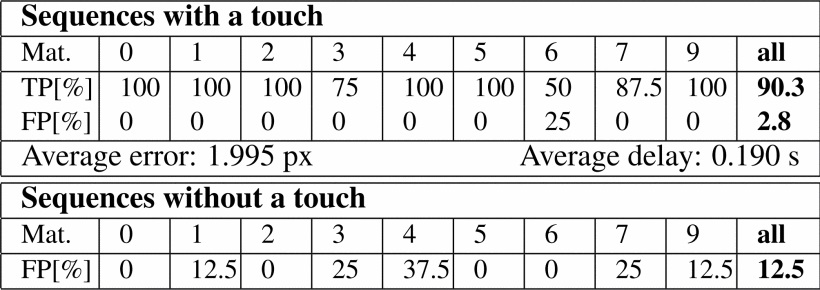
\includegraphics[width=8.5cm, height=3cm]{TouchData}
	\caption{Evaluation results: true positive (TP) and false positive (FP) touch detection on the test data set with different materials (mat.) \cite{Thermal}}
	\label{fig:TouchData}
\end{figure}


\subsection{Thermal Detection}
\label{Thermal Detection}
The two main obstacles that Kurz brings us is detecting the touch in thermal imaging and being able to find where the touch occurred on a 3D object. First he explored temperature profiles of a surface being touched, obstructed, or not interacted with at all. The 4 cases of temperatures profiles are: Object only, Hand only, obstruction by hand, and touch by hand. Object only is just using the cameras to measure the relative constant temperature of an object. Hand only measured the temperature of a hand expecting moderate temperature changes. Obstruction by hand starts with detecting an object having a hand come between the object and the camera, not touching the object. The infrared will detect the rapid change from cool surface to a warm body then rapidly back to the cool surface. Touch by hand is when the object is actually touched. For the temperature it will start with the cool surface the warm body obstructs the area then once the hand moves away instead of a rapid change back to a cool surface there is a rapid decrease to a temperature between that of the hand and the object. After the rapid decrease the area will slowly cool, reverting to the starting temperature. 
 
\(
\begin{matrix}
 t_{1}=(1-{1\over 16})t_{ min}+{1\over 16}t_{ max} & t_{2}=(1-{3\over 8})t_{ min}+{3\over 8}t_{ max}\cr a_{1}=0.32{\rm cm}^{2} & a_{2}=1.54{\rm cm}^{2}
 \end{matrix}
\)

Above is the OpenCV SimpleBlobDetector that Kurz used to calculate the sized of the thermal fingerprints left on the object. \(t_1\) and \(t_2\) is the temperature range the thermal camera is looking for when to detect if an object was touched. \(a_1\) and \(a_2\) is the area range that is used for detecting the blobs. Blobs are the set of circular areas returned by OpenCV's SimpleBlobDetector. Ignoring blobs with centers close to 10 pixels to the edge of the image, this is to reduce the amount of false positives from fingers entering and leaving the image. Kurz's experiments focused on single touch events, ignoring all blobs if there are multiple.        


\subsection{Materials Tested}
\label{Materials Tested}
The blob detector is designed to handle objects that differ in material and temperature. This should also work for different users that have differing finger or body temperatures, also the touch time and pressure would most likely be different. Kurz tested the algorithm with an array of materials one would encounter everyday. This consisted of different applicants touching different surfaces at different temperatures \cite{3D}. Figure \ref{fig:ThermalTest} is the testing environment Kurz used to test different materials. The materials tested are paper, plastics, glass, and metal. Being placed on the table centered with the camera, and the camera is 300 mm from the table top. Using four different people in a controlled office environment with ambient temperature at \(25^o\)C. A different group of four people did the same experiment, but outside in temperature of \(12^o\)C. Leaving the test samples in the environment that they would be tested in for around thirty minutes to ensure they conformed to the environments temperature. The test consisted of having the person first pass their hand between the material and the camera, not touching the material. After that they were told just to touch the middle of the material as if it were a key on a keyboard. Notably it was not specified which finger to use and how to have the finger leave the object, leaving that entirely up to the subject. After this test was done Kurz had around 400 thermal images with a time stamp and labeled according to the action, material and testers name. The results of the tests ran showed that number 8, steel, from figure \ref{Materials Tested} does not work well with thermal interaction. This is due to the high rate at which steel dissipates heat, making it difficult to detect using their method. The data collected on steel was removed from figure \ref{fig:TouchData}. Out of the remaining 9 material sequences only two detected a touch in the wrong area. Material 6, glass, from the outside tests had these false positives because the sticker appears warmer then the glass outdoors. 7 sequences could not detect touch due to the short period of contact. The false positives in the sequences without touch in figure \ref{fig:TouchData} were quite high. This was attributed to residual heat left during the placement of the material under the camera. 

\subsection{Applications}
\label{Applications}

\begin{figure}
	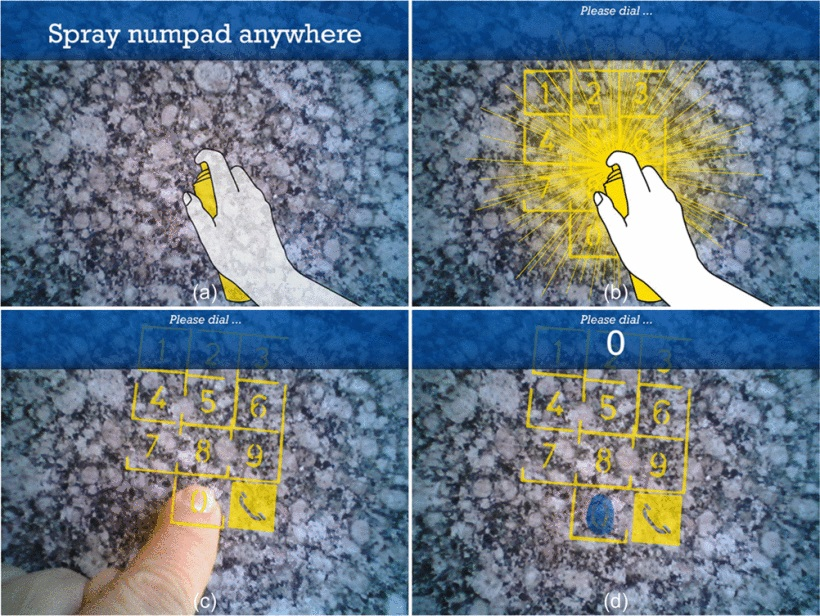
\includegraphics[width=8cm, height=8cm]{numpad}
	\caption{A number pad on a granite countertop seen through the screen of the mobile device \cite{Thermal}.}
	\label{fig:numpad}
\end{figure}

Since the prototype was a more of a hand held device Kurz focuses on wearable technology and head-mounted displays when no touch screens are available. Two of the main applications mentioned in the paper are Spray-On GUI's and augmented floor plans. Spray-On GUI's utilizes any surface available to you, an example would be a granite countertop (see figure \ref{fig:numpad}). Calling it instance tracking, which creates an image and can track it. The camera can move around freely and the object remains in one place. When one of the keys is touched the camera is able to determine the corresponding key that was touched bales on the location in the thermal image. The AR floor plans is where there is a printed floor plan of a building, lets say a mall. That allows the user to press the desired location on floor plan that would display information of the shop or location pressed, such as name, business hours, ratings, and contact information. With this approach there would be not need for a Spray-on GUI since the camera would use the shapes of the floor plan in lieu of virtual buttons.          


\section{3D Data Visualization}
\label{sec:3D Data Visualization}
I will now focus on a paper that explores the use of SAR as a tool for 3D data visualization. As we know from Section \ref{sec:Spatial Augmented Reality}, SAR uses projectors to augment what is already there. Thomas et al. \cite{3D} focus more on 3D data visualization, and not manipulation. Being able to see and touch the data is their main focus. Pushing the idea that using multiple inputs, sight and touch, to help you remember the data being displayed. They \cite{3D} define their proposed use of SAR as a tool for 3D visualization in following ways. First they propose the use of SAR to benefit user's ability to see, understand, and manipulate 3D visualization data. Second is the tabletop SAR prototype that is able to demonstrate many possibilities. Figure \ref{fig:Tabletop}  is an image of their prototype tabletop SAR system. The projections on the physical props define areas of investigation in a 3D volume. The 4K monitor provides detail views of the data in a 2D space. Third is the large applications of SAR, called \textit{CAVE} it is discussed later in this section.


\subsection{Visualizing Data}
\label{sec:Visualizing Data}
Data visualization is the representation of data visually. Some basic examples would be pie charts, scatter-plots, bar charts, and the can list goes on. Data visualization can be used in any field, from showing the demographic of a neighborhood to displaying how many shooting stars happen over the course of a year. Visualizing data is also an effective way to show information quickly and efficiently. Humans tend to recall pictures easier than words. That is why there are many different types of charts. As mentioned in \ref{sec:Data Visualization}, the wide range of the types of data you can visualize makes what the papers proposes versatile in the real world.      


\begin{figure}
	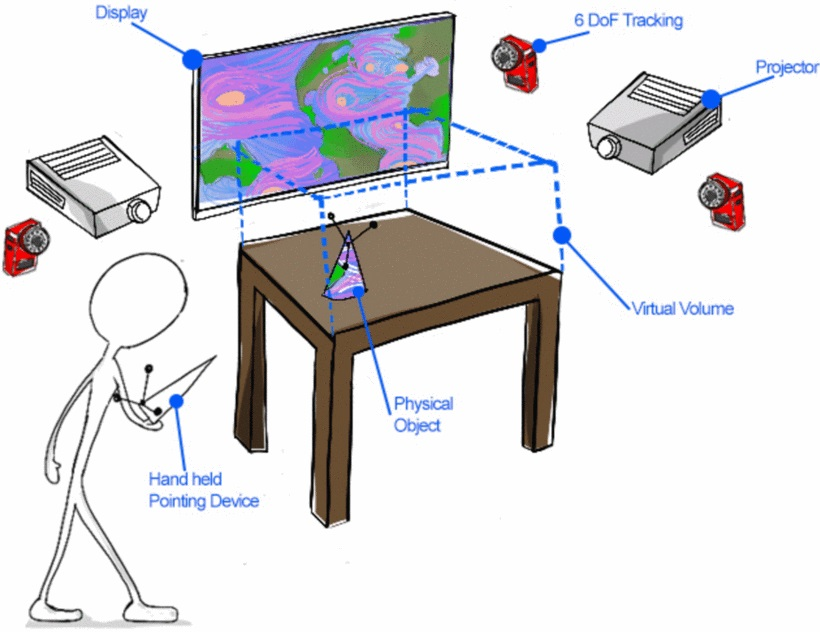
\includegraphics[width=8.5cm, height=5cm]{Tabletop}
	\caption{Tabletop setup \cite{3D}}
	\label{fig:Tabletop}
\end{figure}
\subsection{Applications}
\label{sec:Applications}

The paper mentions two ways that 3D data visualization can be applied in the real world. The main one they mention is the tabletop. This is a proposed system where there is a 2D display, they call it a fish tank view, a table with the physical object(s), the virtual volume, the hand held pointing device, 6DOF trackers, and the projectors. The virtual volume is the space around the table top, starting from the surface of the table extending up a foot or two. 

The CAVE is larger scale version of the tabletop method. Using walls as the physical objects to project onto. This would require a lot more space, 6DOF tracers, and projectors to get it set up. The benefit the cave model is being able to increase the number of collaborators/viewers. Figure \ref{fig:Cave} is one of a couple CAVE variations possible with this technology.

\subsection{Limitations}
\label{sec:Limitations}

The initial experimentation with Thomas et al. \cite{3D} prototype showed a number of limitations with the approach they took. The first is that the lighting the room must be controlled, as details in the gradients of the projected data may be lost with too much ambient lighting. Like anything projector related it works best in dim to dark room/places, depending on the type of projector. Normally we would not take a projector outside in the middle of the day and try to use it. Even inside can be too bright, teachers tend to shut off the lights closest to the screen when they use a projector. \cite{3D} mention that depending on the ambient lighting in the room one possible solution would be upgrading to a more powerful projector.

\subsection{Conclusion}
\label{sec:Conclusion}

The goal of Thomas et al. \cite{3D} was presenting SAR as a tool to enrich the process of 3D visualization. They layout their plan on using SAR with these three points. One is purposed features to benefit the use's abilities interpret the data. The second point being the example of a tabletop prototype (see figure \ref{fig:Tabletop}) showing the flexibility of this as a 3D visualization tool. Lastly the larger scale CAVE applications as ways to increase possible collaboration size.      


\begin{figure}
	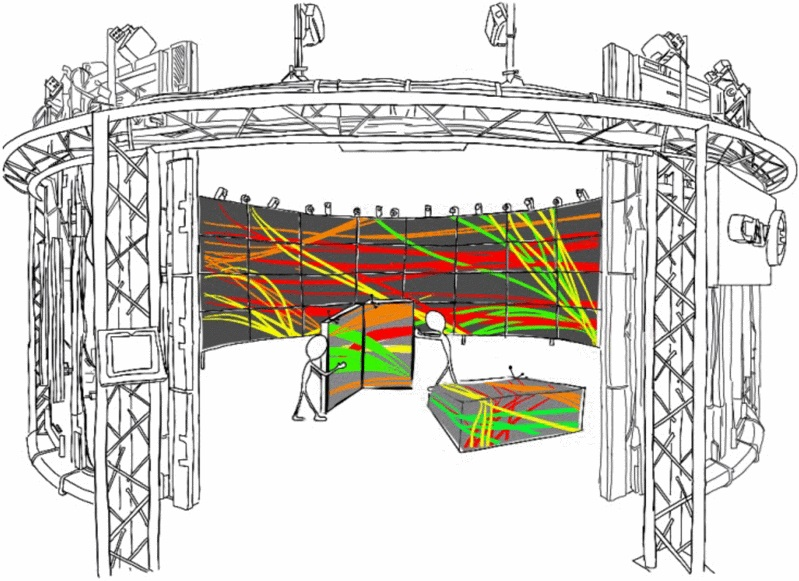
\includegraphics[width=8.5cm, height=5cm]{Cave}
	\caption{One of the CAVE systems mentioned by Thomas et al. \cite{3D}}
	\label{fig:Cave}
\end{figure}  


\section{Joining Together}
\label{sec:Joining Together}
Both sections \ref{sec:Thermal Interaction} and \ref{sec:3D Data Visualization} were fascinating papers papers to read. Reading them both in one day got me thinking of the possibility of mixing those two approaches. In section \ref{sec:3D Data Visualization} a 6DOF object is needed to track ones position, but with the Thermal Interactions section, \ref{sec:Thermal Interaction}, the camera is able to detect positions of objects using viable light cameras.  

\subsection{Strengths and Weaknesses}
\label{Strengths and Weaknesses}

\subsection{Applications}
\label{Applications}

\subsection{Conclusion}
\label{Conclusion}

\section{Alternate Interactions}
\label{sec:Alternate Interactions}

\section{Acknowledgments}
\label{sec:Acknowledgments}

\bibliographystyle{abbrv}
\bibliography{annotatedBibliography}

\end{document}